\documentclass{paper}
\usepackage{times}
\usepackage{geometry}
\geometry{letterpaper, portrait, margin=1in}
\usepackage[utf8]{inputenc}
\usepackage{enumitem,amssymb}
\usepackage{ragged2e}
\usepackage{physics}
\usepackage{siunitx}
\usepackage{float}
\usepackage{mathtools}
\usepackage{amsmath}

\usepackage{caption}
\usepackage[hidelinks]{hyperref}
\usepackage{url}

\usepackage{pgfplots}
\usepackage{graphicx}
\usepackage{epstopdf}
\graphicspath{{data/cos-w7}}

\usepackage{biblatex}
\bibliography{refs}

\title{cos-w7 tasks}
\author{ariahayd}
\date{15 March 2022}

\begin{document} 

\maketitle

\begin{enumerate}
    \item % 1.
      The relationship between time and temperature during the radiation
      dominated era of the universe is given by:
      \[
        t = \left(\frac{T}{\SI{1.5e10}{K}}\right)^{-2}\si{s} \implies
        T = \frac{\SI{1.5e10}{K}}{\sqrt{t}}
      \]

      Where \(t=\SI{1e-6}{s}\), \(T=\SI{1.5e13}{K}\). A particle with mass
      behaves like radiation when in thermal equilibrium and when at 
      relativistic energies. This model can be applied at temperatures
      greater than \(10^{13}\si{K}\) and as far back as the point at which
      quantum gravity becomes significant among the forces.

      The particles that can be created at this temperature is given by:
      \[
        E = m c^2 = K T = \SI{1.29e9}{eV} \approx M_p = \SI{938}{MeV}
      \]

      Nuclear synthesis occurred shortly after the quark-hadron
      (\(10^{29}-10^{13}\si{K}\)) and lepton (\(10^{13}-10^{10}\si{K}\)) eras,
      producing atomic nuclei.

    \item % 2.
      Photons dominate present day radiation density, but neutrinos have a 
      significant contribution as well. Theory describes non-interacting,
      non-annihilating neutrinos created during the lepton era. This has not
      been detected, but is considered to have a similar number density as
      cosmic microwave background photons because, like photons, a neutrino
      does not annihilate with its antiparticle and so streams freely.

    \item % 3.
      The number density of baryons is a not a conserved quantity in general, 
      but during the nucleosynthesis era of the early universe, the 
      characteristic stabilty of neutrons was long enough to conserve the
      abundances of neutrons within nuclei antecursors deuterium and helium.
      \begin{figure}[!hbt]
        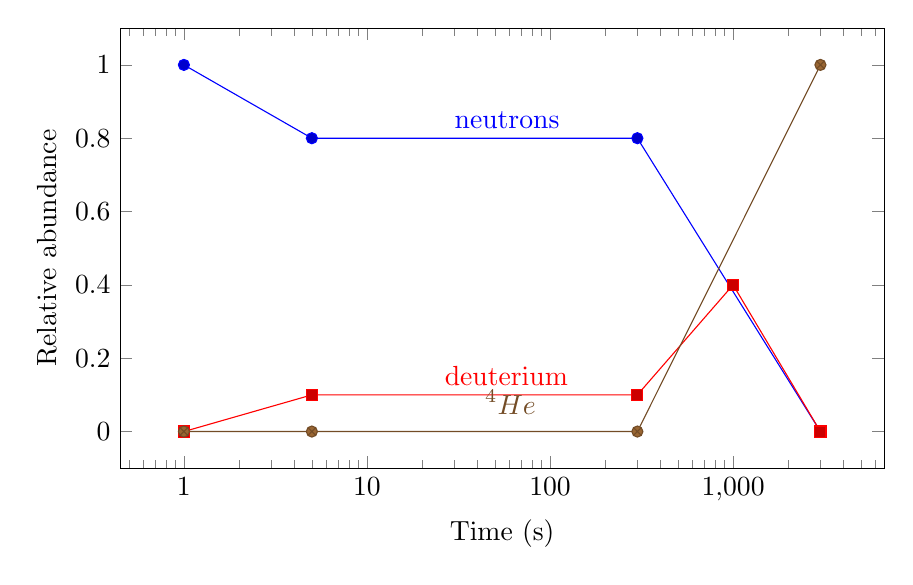
\begin{tikzpicture}
          \begin{axis}[
              height=0.2\paperheight,
              width=0.8\linewidth,
              scale only axis,
              xlabel={Time (s)}, 
              ylabel={Relative abundance},
              xmode=log,
              log ticks with fixed point,
            ]
            \addplot table {
              1 1
              5 0.8
              300 0.8
              3000 0
            } node[above,pos=.5] {neutrons};
            \addplot table {
              1 0
              5 0.1
              300 0.1
              1000 0.4
              3000 0
            } node[above,pos=.5] {deuterium};
            \addplot table {
              1 0
              5 0
              300 0
              3000 1
            } node[above,pos=.5] {\(\prescript{4}{}{He}\)};
          \end{axis}
        \end{tikzpicture}
        \label{fig:mass-fractions}
        \caption{Relative abundances of neutrinos, deuterium, and 
          \(\prescript{4}{}{He}\) over time}
      \end{figure}

    \item %4
      Nucleosynthesis does not occur in a significant way until the long tail
      of energetic photons is diffuse enough to overcome the ``deuterium
      bottleneck.'' Before \(\SI{3e9}{K}\), the universe contained a 
      sufficient number of high energy photons to prevent the combination of
      proton and neutron particles (deuterium) for long enough timescales to
      form larger nuclei. Because deuterium is the most fundamental nucleous,
      the process of nucleosynthesis was halted.

      The neutron-proton ratio is governed by the equilibrium temperature 
      before the nucleosynthesis era. The neutron is slightly heavier than the 
      proton so is less likely to occur at a given single temperature.

      Before nucleosynthesis, the ratio of protons to neutrons was goverened
      by the cross-sectional interactions of neutrons and positrons and
      neutrinos to form protons. At \(T=10^{10}\si{K}\), the timescale of
      interactions of the weak nuclear force to cause neutron transitions is
      much less than the timescale for decreasing particle density. The
      decrease in density at \(T=10^{10}\si{K}\) makes neutron transitions 
      much less likely, freezing the ratio of protons to neutrons.

      During the nucleosynthesis era, neutrons and protons combine to form
      He-4 and heavier elementary nuclei through the deuterium intermediate.
      All free neutrons are consumed through this combination, while the
      excess of protons goes unused, causing the ratio of protons to neutrons
      to grow extremely.

      The reaction \(2n + 2p \rightarrow \prescript{4}{}{He}\) is not likely to spontaneously
      occur because it is a 4-body reaction and all four constituents are
      unlikely to be within the same interaction cross-section at the same
      time.

      \(\prescript{4}{}{He}\) is formed through these reactions:
      \begin{equation}
        \begin{split}
          p + n \rightarrow \prescript{3}{}{He} + \gamma          \\
          \prescript{2}{}{He} + \prescript{2}{}{He} \rightarrow   
            \prescript{3}{}{He} + p | n     \\
          \prescript{3}{}{He} + \prescript{2}{}{He} \rightarrow   
            \prescript{4}{}{He} + n | p
        \end{split}
      \end{equation}

      This chain is a series of 2-body reactions limited by the prevalence
      of neutrons, which has an initial mass fraction of 226 per 1000 protons
      (see 29.2 of Carroll-Ostlie\cite{Carroll-Ostlie}). When all free 
      neutrons are exhausted, \(\prescript{4}{}{He}\) makes up about 25\% of 
      the baryonic mass.

    \item %5
      If the timescale for decomposition of free neutrons was one minute 
      rather than ten minutes, the mass fraction of neutrons available for
      nucleosynthesis would be decreased by a factor of:
      \[
        \frac{n}{n+p} \approx 0.18 \exp{\frac{-300\si{s}}{60\si{s}}} = 0.0012
      \]
      
      This is a reduction from the modeled mass fraction of:
      \[
        \frac{n}{n+p} \approx 0.18 \exp{\frac{-300\si{s}}{600\si{s}}} = 0.11
      \]

      Many fewer neutrons would be available for combination into He-4 
      because so many would have decayed before the time of a temperature low
      enough for deuterium to become stable and to be part of the reaction
      chain. This would result in a \(\prescript{4}{}{He}\) mass fraction 0.01 
      of the current hot big bang model, or 25\% of the total baryonic mass.

    \item %6
      \(\Omega_{baryons}\) is the density parameter due to all baryons (bound
      quarks) and, for simplicity, the electron leptons as well. A
      calculation of the atomic nuclei produced through BBN infers the amount
      of energy captured as baryons from a primordial source. This can be
      validated with measurements of how the mass fractions of ``local'' stars
      deviate from the BBN model to determine how much primordial material
      has been processed.

    \item %7
      The difficulty with measure the baryonic density of the universe from
      the direct, current day measurements is that the primordial material
      has been processed so the ratios of bound nuclei deviate from what
      was produced only through BBN.
      
\end{enumerate}

This paper is available publicly.\cite{Hayden_Cosmology_Source_Repo}

\pagebreak
\printbibliography

\end{document}

